\documentclass[reprint,amsmath,amssymb,aps]{revtex4-2}
\usepackage{balance}
\usepackage[%
    margin=10mm,% ако не си принтира 10мм не изглежда грозно, а може да събереш повече текст
    % showframe=true,%
    ]{geometry}
\usepackage[T1,T2A]{fontenc}
\usepackage[utf8]{inputenc}
\usepackage[main=bulgarian, english]{babel}
\usepackage{float}
\AtBeginDocument{\selectlanguage{bulgarian}}
\newcommand{\degree}{^{\circ}}
\usepackage{amsmath}
\usepackage{graphics}
\usepackage{graphicx}
\graphicspath{{.}}
\newcommand{\abs}[1]{\lvert#1\rvert}
\let\phi\varphi
\usepackage{booktabs} % от тук се използва само \midrule може и без него 
\usepackage{dcolumn}
\usepackage{lipsum}
\newcolumntype{d}[1]{D{.}{.}{#1}}
\usepackage[unicode=true,pdfusetitle]{hyperref}
\usepackage[]{siunitx}

\usepackage[compact]{titlesec}

\begin{document}
\setlength{\abovedisplayskip}{3pt}
\setlength{\belowdisplayskip}{3pt}    

\title{Топлопроводност на слабопроводящи материали}

\author{Васил Николов}
\date{26.04.2022}
\maketitle


\section{Цел на упражнението}

Да се определи коефициентът на топлопроводност на тънък дискообразен образец. 


\section{Експериментална установка}

Установката се състои от нагревател и охладител, чиито температури се мерят електронно, и тънък цилиндричен образец, чийто коефициент на топлопроводност искаме да намерим. Нагревателят и охладителят са медни плочи с диаметърът на образеца. На нагряващата плоча (отгоре на установката) е прикачен реотан, а под охлаждащата плоча (отдолу на установката) има вентилатор. 

Експериментът се състои от две части. В първата част задаваме температура на нагревателя, при която искаме да постигнем стационарно състояние, и измерваме крайната температура на охладителната плоча $T_2$. Във втората част нагряваме охладителната плоча до температура, по-висока от тази при стационарното състояние от част 1, и целим да измерим колко бързо се охлажда. За да го постигнем нагряваме охладителя до температура около $10\circ \ C$ по-висока от $T_2$, махаме нагревателя и оставяме охладителя да излъчва топлината си, като мерим на всеки $\Delta t = 10 \ \si{s}$. След това числено намираме производната на температурата от времето в точката, където температурата е равна на $T_2$. Важно е да се отбележи, че тъй като в този случай охладителят излъчва от страничната си стена и и двете си основи производната на температурата му по времето ще е по-висока. 


\section{Теоретична обосновка}
\subsection{Достигане на стационарно състояние}

Нека при достигнатото стационарно състояние температурата на нагревателя е $T_1$, а на охладителя - $T_2$. Тогава можем да запишем законът на Фурие в следният вид:

\begin{equation*} \label{eq:1}
    P_1 = k\frac{T_1 - T_2}{h} \pi R^2 \tag{1}
\end{equation*}

Тук $h$ е височината на диска, $R$ е радиусът му, а $k$ е коефициентът на топлопроводност на материала. $P_1$ е мощността, която охладителят излъчва при температура $T_2$, през страничната си стена и долната си основа.

\subsection{Измерване на скорост на охлаждане на охладителя}

Можем да изразим мощността, която охладителят излъчва със следната формула: 

\begin{equation*} \label{eq:2}
    P_2 = m c \frac{dT}{dt} \tag{2}
\end{equation*}

Тук $m$ е масата на охладителната плоча, а $c$ е специфичният топлинен капацитет на медта. Освен това можем да запишем и следното равенство за мощностите, излъчвани от охладителя в двете части на експеримента: 

\begin{equation*} \label{eq:3}
    \frac{P_2(T_2)}{P_1(T_2)} = \frac{2\pi R^2 + 2\pi Rh}{\pi R^2 + 2\pi Rh} = \frac{S_2}{S_1} \tag{3}
\end{equation*}

Това е защото във втората част охладителят излъчва през цялата си площ, а в първата - само през страничната си стена и долната основа. Комбинирайки уравнения \eqref{eq:1}, \eqref{eq:2} и \eqref{eq:3} получаваме 

\begin{align*}
    \frac{dT}{dt} \frac{mc h}{k (T_1 - T_2) \pi R^2} = \frac{S_2}{S_1} \\
    k = \frac{dT}{dt} \frac{mc h ( R^2 + 2 Rh)}{(T_1 - T_2) (2 R^2 + 2 Rh) \pi R^2} \label{eq:4} \tag{4}
\end{align*}

По уравнение \eqref{eq:4} ще пресметнем коефициентът на топлопроводност на образеца. 

\section{Експериментални данни и резултати}
\subsection{Достигане на стационарно състояние}

За конкретната установка стационарното състояние се достига за около $15 \ \si{min}$. От графиката на Фигура \ref{fig:1} температурите на нагревателя и охладителя можем да видим крайните им стойности, $T_2 = (55.0 \pm 0.1) \degree C$ и $T_1 = (44.1 \pm 0.1) \degree C$. 

\begin{figure}[H] 
    \centering
    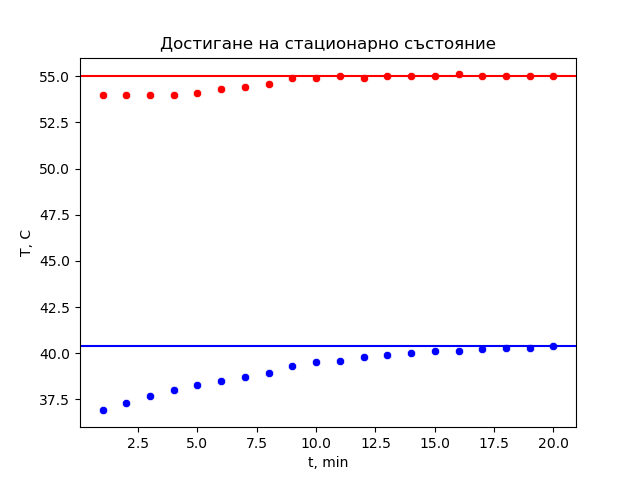
\includegraphics[width=\columnwidth, keepaspectratio=true]{graph_statz.png}
    \caption{}
    \label{fig:1}
\end{figure}

\subsection{Измерване на скоростта на охлаждане на охладителя}

На Фигура \ref{fig:2} е представена температурата на охладителя като функция на времето. За да намерим нейната числена производна в точката, където температурата е числено равна на $T_2 = 40.4 \ \degree C$ фитираме полином от пета степен на експерименталните данни, и намираме аналитично неговата производна.  

\begin{figure}[ht]
    \centering
    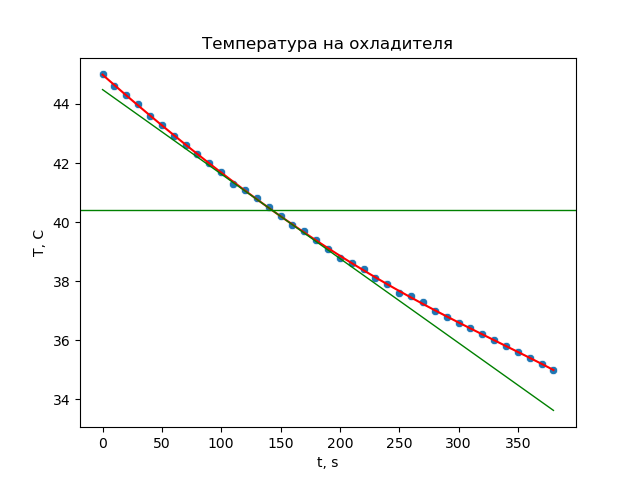
\includegraphics[width=\columnwidth, keepaspectratio=true]{graph_cool.png}
    \caption{} 
    \label{fig:2}
\end{figure}

Използвайки формула \eqref{eq:4} пресмятаме крайната стойност за коефициенът на топлопроводност на образеца - $k = 0.11 \ \si{Wm^{-1}K^{-1}} \pm 3\%$.  За да се пресметне грешката се предполага, че грешката в производната на температурата е около $1\%$. Този резултат е очакван - топлопроводимостта на образеца е от същия порядък като тази на плексиглас. 

\end{document}











